%%%% Paramétrage du TD %%%%
\def\xxactivite{ \ifprof \normalsize{Application 1 -- Corrigé } \else  Application 1 \fi} % \normalsize \vspace{-.4cm}
\def\xxauteur{\textsl{Xavier Pessoles}}


\def\xxnumchapitre{Chapitre 1 \vspace{.2cm}}
\def\xxchapitre{\hspace{.12cm} Équilibrage des solides en rotation}

\def\xxcompetences{%
%\textsl{%
%\textbf{Savoirs et compétences :}\\
%\begin{itemize}[label=\ding{112},font=\color{ocre}] 
%\item \textit{Res1.C2} : principe fondamental de la dynamique;
%\item \textit{Res1.C1.SF1} : proposer une démarche permettant la détermination de la loi de mouvement.
%\end{itemize}
%}
}

\def\xxtitreexo{Application 01}
\def\xxsourceexo{\hspace{.2cm} \footnotesize{Éditions Vuibert}}

\def\xxfigures{
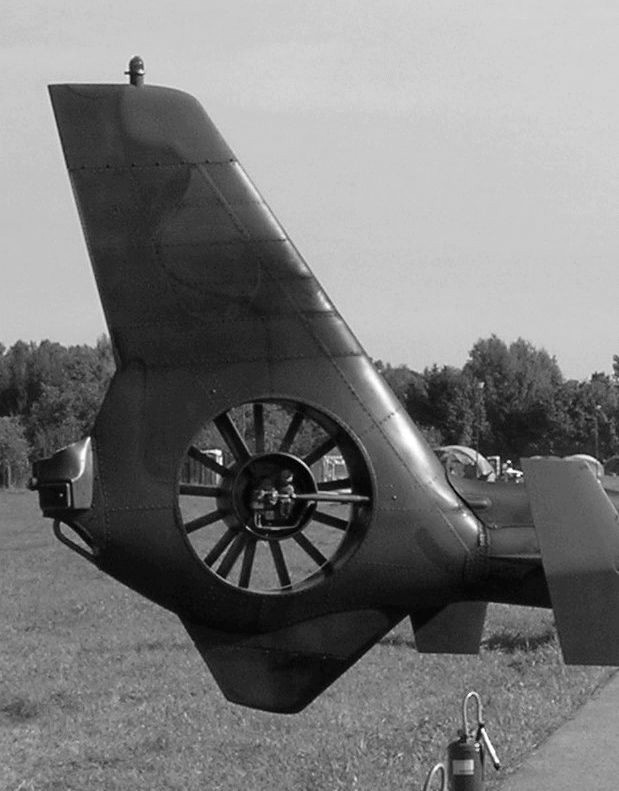
\includegraphics[width=.4\linewidth]{fig_00}
}%figues de la page de garde


\iflivret
\pagestyle{empty}


%%%%%%%% PAGE DE GARDE COURS
\ifcours
% ==== BANDEAU DES TITRES ==== 
\begin{tikzpicture}[remember picture,overlay]
\node at (current page.north west)
{\begin{tikzpicture}[remember picture,overlay]
\node[anchor=north west,inner sep=0pt] at (0,0) {\includegraphics[width=\paperwidth]{\thechapterimage}};
\draw[anchor=west] (-2cm,-8cm) node [line width=2pt,rounded corners=15pt,draw=ocre,fill=white,fill opacity=0.6,inner sep=40pt]{\strut\makebox[22cm]{}};
\draw[anchor=west] (1cm,-8cm) node {\huge\sffamily\bfseries\color{black} %
\begin{minipage}{1cm}
\rotatebox{90}{\LARGE\sffamily\textsc{\color{ocre}\textbf{\xxnumpartie}}}
\end{minipage} \hfill
\begin{minipage}[c]{14cm}
\begin{titrepartie}
\begin{flushright}
\renewcommand{\baselinestretch}{1.1} 
\Large\sffamily\textsc{\textbf{\xxpartie}}
\renewcommand{\baselinestretch}{1} 
\end{flushright}
\end{titrepartie}
\end{minipage} \hfill
\begin{minipage}[c]{3.5cm}
{\large\sffamily\textsc{\textbf{\color{ocre} \discipline}}}
\end{minipage} 
 };
\end{tikzpicture}};
\end{tikzpicture}
% ==== FIN BANDEAU DES TITRES ==== 


% ==== ONGLET 
\begin{tikzpicture}[overlay]
\node[shape=rectangle, 
      rounded corners = .25 cm,
	  draw= ocre,
	  line width=2pt, 
	  fill = ocre!10,
	  minimum width  = 2.5cm,
	  minimum height = 3cm,] at (18.3cm,0) {};
\node at (17.7cm,0) {\rotatebox{90}{\textbf{\Large\color{ocre}{\classe}}}};
%{};
\end{tikzpicture}
% ==== FIN ONGLET 


\vspace{3.5cm}

\begin{tikzpicture}[remember picture,overlay]
\draw[anchor=west] (-2cm,-6cm) node {\huge\sffamily\bfseries\color{black} %
\begin{minipage}{2cm}
\begin{center}
\LARGE\sffamily\textsc{\color{ocre}\textbf{\xxactivite}}
\end{center}
\end{minipage} \hfill
\begin{minipage}[c]{15cm}
\begin{titrechapitre}
\renewcommand{\baselinestretch}{1.1} 
\Large\sffamily\textsc{\textbf{\xxnumchapitre}}

\Large\sffamily\textsc{\textbf{\xxchapitre}}
\vspace{.5cm}

\renewcommand{\baselinestretch}{1} 
\normalsize\normalfont
\xxcompetences
\end{titrechapitre}
\end{minipage}  };
\end{tikzpicture}
\vfill

\begin{flushright}
\begin{minipage}[c]{.3\linewidth}
\begin{center}
\xxfigures
\end{center}
\end{minipage}\hfill
\begin{minipage}[c]{.6\linewidth}
\startcontents
%\printcontents{}{1}{}
\printcontents{}{1}{}
\end{minipage}
\end{flushright}

\begin{tikzpicture}[remember picture,overlay]
\draw[anchor=west] (4.5cm,-.7cm) node {
\begin{minipage}[c]{.2\linewidth}
\begin{flushright}

\includegraphics[width=2cm]{logoCC}
\end{flushright}
\end{minipage}
\begin{minipage}[c]{.2\linewidth}
\textsl{\xxauteur} \\
\textsl{\classe}
\end{minipage}
 };
\end{tikzpicture}

\newpage
\pagestyle{fancy}

%\newpage
%\pagestyle{fancy}

\else
\fi
%% FIN PAGE DE GARDE DES COURS

%%%%%%%% PAGE DE GARDE TD
\iftd
%\begin{tikzpicture}[remember picture,overlay]
%\node at (current page.north west)
%{\begin{tikzpicture}[remember picture,overlay]
%\draw[anchor=west] (-2cm,-3.25cm) node [line width=2pt,rounded corners=15pt,draw=ocre,fill=white,fill opacity=0.6,inner sep=40pt]{\strut\makebox[22cm]{}};
%\draw[anchor=west] (1cm,-3.25cm) node {\huge\sffamily\bfseries\color{black} %
%\begin{minipage}{1cm}
%\rotatebox{90}{\LARGE\sffamily\textsc{\color{ocre}\textbf{\xxnumpartie}}}
%\end{minipage} \hfill
%\begin{minipage}[c]{13.5cm}
%\begin{titrepartie}
%\begin{flushright}
%\renewcommand{\baselinestretch}{1.1} 
%\Large\sffamily\textsc{\textbf{\xxpartie}}
%\renewcommand{\baselinestretch}{1} 
%\end{flushright}
%\end{titrepartie}
%\end{minipage} \hfill
%\begin{minipage}[c]{3.5cm}
%{\large\sffamily\textsc{\textbf{\color{ocre} \discipline}}}
%\end{minipage} 
% };
%\end{tikzpicture}};
%\end{tikzpicture}

%%%%%%%%%% PAGE DE GARDE TD %%%%%%%%%%%%%%%
%\begin{tikzpicture}[overlay]
%\node[shape=rectangle, 
%      rounded corners = .25 cm,
%	  draw= ocre,
%	  line width=2pt, 
%	  fill = ocre!10,
%	  minimum width  = 2.5cm,
%	  minimum height = 2.5cm,] at (18.5cm,0) {};
%\node at (17.7cm,0) {\rotatebox{90}{\textbf{\Large\color{ocre}{\classe}}}};
%%{};
%\end{tikzpicture}

% PARTIE ET CHAPITRE
%\begin{tikzpicture}[remember picture,overlay]
%\draw[anchor=west] (-1cm,-2.1cm) node {\large\sffamily\bfseries\color{black} %
%\begin{minipage}[c]{15cm}
%\begin{flushleft}
%\xxnumchapitre \\
%\xxchapitre
%\end{flushleft}
%\end{minipage}  };
%\end{tikzpicture}

% BANDEAU EXO
\iflivret % SI LIVRET
\begin{tikzpicture}[remember picture,overlay]
\draw[anchor=west] (-2cm,-3.3cm) node {\huge\sffamily\bfseries\color{black} %
\begin{minipage}{5cm}
\begin{center}
\LARGE\sffamily\color{ocre}\textbf{\textsc{\xxactivite}}

\begin{center}
\xxfigures
\end{center}

\end{center}
\end{minipage} \hfill
\begin{minipage}[c]{12cm}
\begin{titrechapitre}
\renewcommand{\baselinestretch}{1.1} 
\large\sffamily\textbf{\textsc{\xxtitreexo}}

\small\sffamily{\textbf{\textit{\color{black!70}\xxsourceexo}}}
\vspace{.5cm}

\renewcommand{\baselinestretch}{1} 
\normalsize\normalfont
\xxcompetences
\end{titrechapitre}
\end{minipage}};
\end{tikzpicture}
\else % ELSE NOT LIVRET
\begin{tikzpicture}[remember picture,overlay]
\draw[anchor=west] (-2cm,-4.5cm) node {\huge\sffamily\bfseries\color{black} %
\begin{minipage}{5cm}
\begin{center}
\LARGE\sffamily\color{ocre}\textbf{\textsc{\xxactivite}}

\begin{center}
\xxfigures
\end{center}

\end{center}
\end{minipage} \hfill
\begin{minipage}[c]{12cm}
\begin{titrechapitre}
\renewcommand{\baselinestretch}{1.1} 
\large\sffamily\textbf{\textsc{\xxtitreexo}}

\small\sffamily{\textbf{\textit{\color{black!70}\xxsourceexo}}}
\vspace{.5cm}

\renewcommand{\baselinestretch}{1} 
\normalsize\normalfont
\xxcompetences
\end{titrechapitre}
\end{minipage}};
\end{tikzpicture}

\fi

\else   % FIN IF TD
\fi


%%%%%%%% PAGE DE GARDE FICHE
\iffiche
\begin{tikzpicture}[remember picture,overlay]
\node at (current page.north west)
{\begin{tikzpicture}[remember picture,overlay]
\draw[anchor=west] (-2cm,-2.25cm) node [line width=2pt,rounded corners=15pt,draw=ocre,fill=white,fill opacity=0.6,inner sep=40pt]{\strut\makebox[22cm]{}};
\draw[anchor=west] (1cm,-2.25cm) node {\huge\sffamily\bfseries\color{black} %
\begin{minipage}{1cm}
\rotatebox{90}{\LARGE\sffamily\textsc{\color{ocre}\textbf{\xxnumpartie}}}
\end{minipage} \hfill
\begin{minipage}[c]{14cm}
\begin{titrepartie}
\begin{flushright}
\renewcommand{\baselinestretch}{1.1} 
\large\sffamily\textsc{\textbf{\xxpartie} \\} 

\vspace{.2cm}

\normalsize\sffamily\textsc{\textbf{\xxnumchapitre -- \xxchapitre}}
\renewcommand{\baselinestretch}{1} 
\end{flushright}
\end{titrepartie}
\end{minipage} \hfill
\begin{minipage}[c]{3.5cm}
{\large\sffamily\textsc{\textbf{\color{ocre} \discipline}}}
\end{minipage} 
 };
\end{tikzpicture}};
\end{tikzpicture}

\iflivret
\begin{tikzpicture}[overlay]
\node[shape=rectangle, 
      rounded corners = .25 cm,
	  draw= ocre,
	  line width=2pt, 
	  fill = ocre!10,
	  minimum width  = 2.5cm,
	  minimum height = 2.5cm,] at (18.5cm,1.1cm) {};
\node at (17.9cm,1.1cm) {\rotatebox{90}{\textsf{\textbf{\large\color{ocre}{\classe}}}}};
%{};
\end{tikzpicture}
\else
\begin{tikzpicture}[overlay]
\node[shape=rectangle, 
      rounded corners = .25 cm,
	  draw= ocre,
	  line width=2pt, 
	  fill = ocre!10,
	  minimum width  = 2.5cm,
%	  minimum height = 2.5cm,] at (18.5cm,1.1cm) {};
	  minimum height = 2.5cm,] at (18.6cm,0cm) {};
\node at (18cm,0cm) {\rotatebox{90}{\textsf{\textbf{\large\color{ocre}{\classe}}}}};
%{};
\end{tikzpicture}

\fi

\else
\fi



\else
\pagestyle{empty}


%%%%%%%% PAGE DE GARDE COURS
\ifcours
% ==== BANDEAU DES TITRES ==== 
\begin{tikzpicture}[remember picture,overlay]
\node at (current page.north west)
{\begin{tikzpicture}[remember picture,overlay]
\node[anchor=north west,inner sep=0pt] at (0,0) {\includegraphics[width=\paperwidth]{\thechapterimage}};
\draw[anchor=west] (-2cm,-8cm) node [line width=2pt,rounded corners=15pt,draw=ocre,fill=white,fill opacity=0.6,inner sep=40pt]{\strut\makebox[22cm]{}};
\draw[anchor=west] (1cm,-8cm) node {\huge\sffamily\bfseries\color{black} %
\begin{minipage}{1cm}
\rotatebox{90}{\LARGE\sffamily\textsc{\color{ocre}\textbf{\xxnumpartie}}}
\end{minipage} \hfill
\begin{minipage}[c]{14cm}
\begin{titrepartie}
\begin{flushright}
\renewcommand{\baselinestretch}{1.1} 
\Large\sffamily\textsc{\textbf{\xxpartie}}
\renewcommand{\baselinestretch}{1} 
\end{flushright}
\end{titrepartie}
\end{minipage} \hfill
\begin{minipage}[c]{3.5cm}
{\large\sffamily\textsc{\textbf{\color{ocre} \discipline}}}
\end{minipage} 
 };
\end{tikzpicture}};
\end{tikzpicture}
% ==== FIN BANDEAU DES TITRES ==== 


% ==== ONGLET 
\begin{tikzpicture}[overlay]
\node[shape=rectangle, 
      rounded corners = .25 cm,
	  draw= ocre,
	  line width=2pt, 
	  fill = ocre!10,
	  minimum width  = 2.5cm,
	  minimum height = 3cm,] at (18.3cm,0) {};
\node at (17.7cm,0) {\rotatebox{90}{\textbf{\Large\color{ocre}{\classe}}}};
%{};
\end{tikzpicture}
% ==== FIN ONGLET 


\vspace{3.5cm}

\begin{tikzpicture}[remember picture,overlay]
\draw[anchor=west] (-2cm,-6cm) node {\huge\sffamily\bfseries\color{black} %
\begin{minipage}{2cm}
\begin{center}
\LARGE\sffamily\textsc{\color{ocre}\textbf{\xxactivite}}
\end{center}
\end{minipage} \hfill
\begin{minipage}[c]{15cm}
\begin{titrechapitre}
\renewcommand{\baselinestretch}{1.1} 
\Large\sffamily\textsc{\textbf{\xxnumchapitre}}

\Large\sffamily\textsc{\textbf{\xxchapitre}}
\vspace{.5cm}

\renewcommand{\baselinestretch}{1} 
\normalsize\normalfont
\xxcompetences
\end{titrechapitre}
\end{minipage}  };
\end{tikzpicture}
\vfill

\begin{flushright}
\begin{minipage}[c]{.3\linewidth}
\begin{center}
\xxfigures
\end{center}
\end{minipage}\hfill
\begin{minipage}[c]{.6\linewidth}
\startcontents
%\printcontents{}{1}{}
\printcontents{}{1}{}
\end{minipage}
\end{flushright}

\begin{tikzpicture}[remember picture,overlay]
\draw[anchor=west] (4.5cm,-.7cm) node {
\begin{minipage}[c]{.2\linewidth}
\begin{flushright}

\includegraphics[width=2cm]{logoCC}
\end{flushright}
\end{minipage}
\begin{minipage}[c]{.2\linewidth}
\textsl{\xxauteur} \\
\textsl{\classe}
\end{minipage}
 };
\end{tikzpicture}

\newpage
\pagestyle{fancy}

%\newpage
%\pagestyle{fancy}

\else
\fi
%% FIN PAGE DE GARDE DES COURS

%%%%%%%% PAGE DE GARDE TD
\iftd
%\begin{tikzpicture}[remember picture,overlay]
%\node at (current page.north west)
%{\begin{tikzpicture}[remember picture,overlay]
%\draw[anchor=west] (-2cm,-3.25cm) node [line width=2pt,rounded corners=15pt,draw=ocre,fill=white,fill opacity=0.6,inner sep=40pt]{\strut\makebox[22cm]{}};
%\draw[anchor=west] (1cm,-3.25cm) node {\huge\sffamily\bfseries\color{black} %
%\begin{minipage}{1cm}
%\rotatebox{90}{\LARGE\sffamily\textsc{\color{ocre}\textbf{\xxnumpartie}}}
%\end{minipage} \hfill
%\begin{minipage}[c]{13.5cm}
%\begin{titrepartie}
%\begin{flushright}
%\renewcommand{\baselinestretch}{1.1} 
%\Large\sffamily\textsc{\textbf{\xxpartie}}
%\renewcommand{\baselinestretch}{1} 
%\end{flushright}
%\end{titrepartie}
%\end{minipage} \hfill
%\begin{minipage}[c]{3.5cm}
%{\large\sffamily\textsc{\textbf{\color{ocre} \discipline}}}
%\end{minipage} 
% };
%\end{tikzpicture}};
%\end{tikzpicture}

%%%%%%%%%% PAGE DE GARDE TD %%%%%%%%%%%%%%%
%\begin{tikzpicture}[overlay]
%\node[shape=rectangle, 
%      rounded corners = .25 cm,
%	  draw= ocre,
%	  line width=2pt, 
%	  fill = ocre!10,
%	  minimum width  = 2.5cm,
%	  minimum height = 2.5cm,] at (18.5cm,0) {};
%\node at (17.7cm,0) {\rotatebox{90}{\textbf{\Large\color{ocre}{\classe}}}};
%%{};
%\end{tikzpicture}

% PARTIE ET CHAPITRE
%\begin{tikzpicture}[remember picture,overlay]
%\draw[anchor=west] (-1cm,-2.1cm) node {\large\sffamily\bfseries\color{black} %
%\begin{minipage}[c]{15cm}
%\begin{flushleft}
%\xxnumchapitre \\
%\xxchapitre
%\end{flushleft}
%\end{minipage}  };
%\end{tikzpicture}

% BANDEAU EXO
\iflivret % SI LIVRET
\begin{tikzpicture}[remember picture,overlay]
\draw[anchor=west] (-2cm,-3.3cm) node {\huge\sffamily\bfseries\color{black} %
\begin{minipage}{5cm}
\begin{center}
\LARGE\sffamily\color{ocre}\textbf{\textsc{\xxactivite}}

\begin{center}
\xxfigures
\end{center}

\end{center}
\end{minipage} \hfill
\begin{minipage}[c]{12cm}
\begin{titrechapitre}
\renewcommand{\baselinestretch}{1.1} 
\large\sffamily\textbf{\textsc{\xxtitreexo}}

\small\sffamily{\textbf{\textit{\color{black!70}\xxsourceexo}}}
\vspace{.5cm}

\renewcommand{\baselinestretch}{1} 
\normalsize\normalfont
\xxcompetences
\end{titrechapitre}
\end{minipage}};
\end{tikzpicture}
\else % ELSE NOT LIVRET
\begin{tikzpicture}[remember picture,overlay]
\draw[anchor=west] (-2cm,-4.5cm) node {\huge\sffamily\bfseries\color{black} %
\begin{minipage}{5cm}
\begin{center}
\LARGE\sffamily\color{ocre}\textbf{\textsc{\xxactivite}}

\begin{center}
\xxfigures
\end{center}

\end{center}
\end{minipage} \hfill
\begin{minipage}[c]{12cm}
\begin{titrechapitre}
\renewcommand{\baselinestretch}{1.1} 
\large\sffamily\textbf{\textsc{\xxtitreexo}}

\small\sffamily{\textbf{\textit{\color{black!70}\xxsourceexo}}}
\vspace{.5cm}

\renewcommand{\baselinestretch}{1} 
\normalsize\normalfont
\xxcompetences
\end{titrechapitre}
\end{minipage}};
\end{tikzpicture}

\fi

\else   % FIN IF TD
\fi


%%%%%%%% PAGE DE GARDE FICHE
\iffiche
\begin{tikzpicture}[remember picture,overlay]
\node at (current page.north west)
{\begin{tikzpicture}[remember picture,overlay]
\draw[anchor=west] (-2cm,-2.25cm) node [line width=2pt,rounded corners=15pt,draw=ocre,fill=white,fill opacity=0.6,inner sep=40pt]{\strut\makebox[22cm]{}};
\draw[anchor=west] (1cm,-2.25cm) node {\huge\sffamily\bfseries\color{black} %
\begin{minipage}{1cm}
\rotatebox{90}{\LARGE\sffamily\textsc{\color{ocre}\textbf{\xxnumpartie}}}
\end{minipage} \hfill
\begin{minipage}[c]{14cm}
\begin{titrepartie}
\begin{flushright}
\renewcommand{\baselinestretch}{1.1} 
\large\sffamily\textsc{\textbf{\xxpartie} \\} 

\vspace{.2cm}

\normalsize\sffamily\textsc{\textbf{\xxnumchapitre -- \xxchapitre}}
\renewcommand{\baselinestretch}{1} 
\end{flushright}
\end{titrepartie}
\end{minipage} \hfill
\begin{minipage}[c]{3.5cm}
{\large\sffamily\textsc{\textbf{\color{ocre} \discipline}}}
\end{minipage} 
 };
\end{tikzpicture}};
\end{tikzpicture}

\iflivret
\begin{tikzpicture}[overlay]
\node[shape=rectangle, 
      rounded corners = .25 cm,
	  draw= ocre,
	  line width=2pt, 
	  fill = ocre!10,
	  minimum width  = 2.5cm,
	  minimum height = 2.5cm,] at (18.5cm,1.1cm) {};
\node at (17.9cm,1.1cm) {\rotatebox{90}{\textsf{\textbf{\large\color{ocre}{\classe}}}}};
%{};
\end{tikzpicture}
\else
\begin{tikzpicture}[overlay]
\node[shape=rectangle, 
      rounded corners = .25 cm,
	  draw= ocre,
	  line width=2pt, 
	  fill = ocre!10,
	  minimum width  = 2.5cm,
%	  minimum height = 2.5cm,] at (18.5cm,1.1cm) {};
	  minimum height = 2.5cm,] at (18.6cm,0cm) {};
\node at (18cm,0cm) {\rotatebox{90}{\textsf{\textbf{\large\color{ocre}{\classe}}}}};
%{};
\end{tikzpicture}

\fi

\else
\fi



\fi
\setlength{\columnseprule}{.1pt}

\pagestyle{fancy}
\thispagestyle{plain}

\ifprof
\vspace{5.5cm}
\else
\vspace{4.9cm}
\fi

\def\columnseprulecolor{\color{ocre}}
\setlength{\columnseprule}{0.4pt} 

%%%%%%%%%%%%%%%%%%%%%%%

\setcounter{exo}{0}


\ifprof
\else
\begin{multicols}{2}



La rotation du rotor de queue d'un hélicoptère est obtenue à partir de la rotation du rotor principal par l'intermédiaire d'un système de transmission. Les arbres n'étant pas parallèles, on utilise un engrenage conique pour assurer cette transmission. Le rotor est donc constitué d'une roue conique standard montée sur un arbre épaulé. L'encastrement des deux pièces n'est pas toujours optimal car l'axe de l'arbre et l'axe de la roue peuvent être décalés de quelques centièmes de millimètres. 
Les opérations de maintenance préventive par contrôle non destructif (CND) correspondant à une analyse vibratoire permettent de détecter ces défauts.

\section*{Cahier des charges}
Un extrait du diagramme des exigences est donné figure suivante.
%Figure \ref{ex_rotor_exigences}.

\begin{center}
%\begin{figure}[!ht]
%\centering
%\includegraphics[width=14cm]{\pathfig/Diagramme_exigences.pdf}
%\includestandalone[width=\linewidth]{\pathfig/Diagramme_exigences}
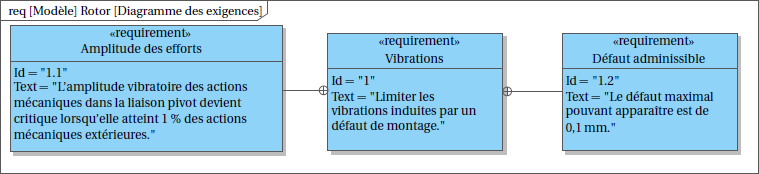
\includegraphics[width=\linewidth]{fig_01}

\textit{Diagramme des exigences pour l'analyse d'un défaut.}
%\caption{Diagramme des exigences pour l'analyse d'un défaut.}
%\label{ex_rotor_exigences}
%\end{figure}
\end{center}


\begin{obj}
L'objectif de l'exercice est de déterminer la relation entre les efforts engendrant des vibrations et le défaut d'alignement des axes. Le diagramme des exigences de la figure précédente %\ref{ex_rotor_exigences} 
définit les critères à respecter.
\end{obj}

\section*{Modéliser le système\\}

%\begin{figure}[!ht]
%\centering
%\includestandalone{\pathfig/modelisation_bis}
%%\includegraphics[width=10cm]{\pathfig/modelisation}
%
%\caption{Modélisation du rotor avec roue conique.}
%\label{ex_rotor_param}
%\end{figure}

\begin{center}
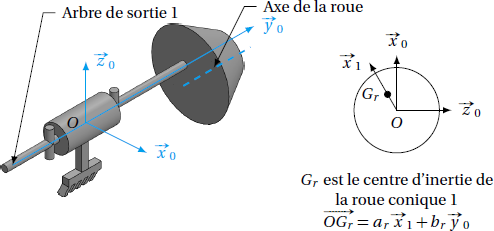
\includegraphics[width=\linewidth]{fig_02}

\textit{Modélisation du rotor avec roue conique.}
\end{center}

On associe un repère $R_1(O,\vect{x_1},\vect{y_0},\vect{z_1})$ à l'arbre en rotation. On note $\theta=(\vect{x_0},\vect{x_1})=(\vect{z_0},\vect{z_1})$ l'angle de rotation autour de l'axe $(O,\vect{y_0})$ de l'ensemble 1 par rapport au bâti fixe 0. La vitesse angulaire est notée $\omega=\dot{\theta}$. 

Le solide 1 est constitué de 2 parties : un arbre de forme cylindrique de centre de gravité $O$, de diamètre $d=\SI{40}{mm}$ et de longueur $2L=\SI{400}{mm}$ et d'une roue conique en forme de tronc de cône plein de largeur $h=\SI{50}{mm}$ (la hauteur du cône correspondant est notée $H$), de diamètre de base $2r_1=\SI{280}{mm}$ et de diamètre de tête $2r_2=\SI{200}{mm}$. Les matériaux des deux pièces sont identiques. Le centre de gravité de la roue conique $G_r$ est tel que $\vect{OG_r}=a_r \vect{x_1}+b_r\vect{y_0}$ avec $a_r$ défaut admissible et $b_r=\SI{425}{mm}$. La masse du tronc de cône est notée $m_r=\SI{20}{kg}$ et celle de l'arbre $m_a=\SI{4}{kg}$ (on note $m=m_r+m_a\approx m_r$ la masse totale de la pièce~1).



\begin{center}
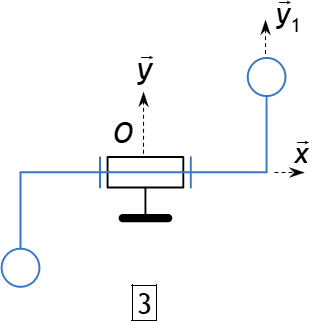
\includegraphics[width=\linewidth]{fig_03}

\textit{Géométrie de la pièce 1 = arbre + tronc de cône.}
\end{center}
%
%
%\begin{figure}[!ht]
%\centering
%%\includegraphics[width=10cm]{\pathfig/rotor}
%\includestandalone{\pathfig/rotor}
%\caption{Géométrie de la pièce 1 = arbre + tronc de cône.}
%%\textcolor{red}{DV : la longueur L va jusqu'au début du tronc de cone de rayon r1. Peut être ajouter la distance selon y0 de O à G1 qui vaut b1. Faire si possible le rayon du cylindre un peu plus petit sur la figure que la largeur h. Allonger l'arbre à gauche pour que le point O soit au milieu (cdg). Mettre aussi H hauteur du cône complet.}
%\label{ex_rotor_geom}
%\end{figure}

\subparagraph{}
\textit{Déterminer le centre de gravité de la pièce 1 : $\vect{OG_1}=a \vect{x_1}+b \vect{y_0}$.}


\section*{Déterminer les actions de liaisons\\}

On prend dans un premier temps une matrice d'inertie quelconque de l'ensemble 1 au point $O$ dans la base $R_1$ : $$\left[I(O,S)\right]=
\begin{bmatrix}
A & -F & -E \\ 
-F & B & -D \\ 
-E & -D & C
\end{bmatrix}_{(\vect{x_1},\vect{y_0},\vect{z_1})}.$$
L'action mécanique extérieure exercée par la denture sur la roue conique est notée : $$\torseurstat{T}{\text{ext}}{1}=\torseurl{X_e \vect{x_1}+Y_e \vect{y_0}+ Z_e \vect{z_1}}{L_e \vect{x_1}+C_e \vect{y_0}+N_e \vect{z_1}}{O}.$$

L'action mécanique exercée dans la liaison pivot parfaite par le bâti 0 est notée : $$\torseurstat{T}{0}{1}=\torseurl{X_0 \vect{x_1}+Y_0 \vect{y_0}+ Z_0 \vect{z_1}}{L_0 \vect{x_1}+ N_0\vect{z_1}}{O}.$$

\subparagraph{}
\textit{Compte tenu de la géométrie de la pièce 1, donner la forme simplifiée de la matrice d'inertie $I_O(S)$.}


\subparagraph{}
\textit{Calculer l'accélération $\vectg{G}{1}{0}$ et le moment dynamique $\vectmd{O}{1}{0}$.}


\subparagraph{}
\textit{Déduire de l'application du PFD les actions mécaniques dans la liaison pivot.}

Pour éviter les vibrations, il faut que les actions mécaniques dans la liaison pivot ne dépendent pas de $\dot{\omega}=\ddot{\theta}$ et de $\omega=\dot{\theta}$.

\subparagraph{}
\textit{Quelles conditions sur la position du centre de gravité et sur la matrice d'inertie doit-on vérifier pour respecter ce critère ?}


\section*{Déterminer les composantes inertielles}

La matrice d'inertie d'un cône de sommet $A$, de rayon $R$, de hauteur $H$ et d'axe $\vect{y}_0$ est la suivante : $\left[I(A,\text{cône})\right]=
\begin{bmatrix}
A_c & 0 & 0 \\ 
0 & B_c & 0 \\ 
0 & 0 & A_c
\end{bmatrix}_{(\vect{x_1},\vect{y_0},\vect{z_1})}
$
avec $A_c=\dfrac{3 m R^2}{20}+\dfrac{3mH^2}{5}$ et $B_c=\dfrac{3mR^2}{10}$.

La masse de ce cône est égale à $\rho \dfrac{\pi H R^2}{3}$ (avec $\rho$ masse volumique). Le centre d'inertie du cône est défini par $\vect{AG_c}=-\dfrac{3 H}{4} \vect{y_0}$.


\subparagraph{}
\textit{Justifier que la matrice d'inertie en $A$ de la roue en forme de tronc de cône défini dans le sujet soit la suivante : $\left[I(A,\text{roue})\right]=\begin{bmatrix}
A_r & 0 & 0 \\ 
0 & B_r & 0 \\ 
0 & 0 & A_r
\end{bmatrix}_{(\vect{x_1},\vect{y_0},\vect{z_1})}
$
avec $A_r=\dfrac{3 m_{c1} r_2^2}{20}+\dfrac{3 m_{c1} H^2}{5} -\dfrac{3 m_{c2} r_2^2}{20}-\dfrac{3 m_{c2} (H-h)^2}{5} $ et $B_r=\dfrac{3 m_{c1} r_1^2}{10}-\dfrac{3 m_{c2} r_2^2}{10}$ où $m_{c1}=\dfrac{\rho \pi r_1^2 H}{3}$ et $m_{c2}=\dfrac{\rho \pi r_2^2 (H-h)}{3}$.}


\subparagraph{}
\textit{Déterminer la matrice d'inertie en $G_r$ de la roue en utilisant le théorème de Huygens puis la déterminer en $O$.}

\subparagraph{}
\textit{Calculer les valeurs numériques de $a$, $b$ et $F$ à partir du cahier des charges, des résultats précédents et des valeurs numériques données en début d'énoncé.}


\section*{Vérification du cahier des charges}

On cherche à déterminer si un défaut admissible défini dans le cahier des charges convient ou non en termes d'efforts vibratoires.
On se place donc en régime permanent ($\dot{\omega}=0$) à la fréquence angulaire de \SI{800}{tr.min^{-1}}. On considère uniquement une action extérieure présentant une résultante selon $\vect{x_1}$ de $X_e=\SI{5000}{N}$ et un moment $N_e$ selon $\vect{z_1}$ égal à $\SI{2000}{Nm}$.


\subparagraph{}
\textit{Calculer la composante de l'action mécanique dans la liaison pivot $X_0$ et le moment $N_0$ pour un défaut maximal (on prendra $H=\SI{86}{mm}$). Conclure quant au cahier des charges.}


\subparagraph{}
\textit{Pourrait-on vérifier les conditions d'équilibrage déterminées dans la première partie avec un petit perçage de masse négative $m_p$ situé en $P$ tel que $\overrightarrow{OP} = a_p \vect{x_1} + b_p \vect{y_0}$.}


\vspace{2cm}

\footnotesize
\begin{enumerate}
\item $a=\frac{m_r a_r}{m}$ et $b=\frac{m_r b_r}{m}$.
\item $D=E=0$.
\item $\vectg{G}{1}{0}=-a\ddot{\theta} \vec{z}_1-a\dot{\theta}^2\vec{x}_1$. $\vectmd{O}{1}{0}=B \ddot{\theta}\vec{y}_0 - F \ddot{\theta} \vec{x}_1 + F \dot{\theta}^2 \vec{z}_1$.


\item $
\left\{ \begin{array}{l}
X_0 + X_e = - m a \dot{\theta}^2 \\
Y_0 + Y_e = 0 \\
Z_0 + Z_e = - m a \ddot{\theta} \\
\end{array}
\right.
\quad
\left\{ \begin{array}{l}
L_0 +L_e = -F \ddot{\theta} \\
C_e = B \ddot{\theta} \\
N_0 +N_e= F \dot{\theta}^2
\end{array}
\right. .
$

\item $a=0$ et $F=0$.

\item .%Le tronc de cône défini dans l'énoncé est obtenu par soustraction de la matrice d'inertie d'un cône de rayon $r_1$ et de hauteur $H$ de sommet $A$ et d'un cône de rayon $r_2$ et de hauteur $H-h$ de sommet $A$.

\item 
$\left[I(O,\text{tronc})\right]=$

$m_r 
\begin{bmatrix}
\frac{A_r}{m_r}-(L+H-b_r)^2+b_r^2 & -a_r(L+H) & 0 \\ 
-a_r(L+H) & \frac{B_r}{m_r} & 0 \\ 
0 & 0 & \frac{A_r}{m_r}+b_r^2-(L+H-b_r)^2
\end{bmatrix}_{(\vect {x_1},\vect{y_0},\vect{z_1})}.$

\item $a=\frac{m_r a_r}{m}=\SI{0.08}{mm}$ et $b=\frac{m_r b_r}{m}=\SI{354}{mm}$.
 $F=m_r\cdot a_r(L+H)=20\times \num{0,1e-3} \times 0,286=\SI{5.7e-4}{kg.m^2}$. 

\item  $X_0=- X_e - m a \omega^2$  et $N_0=-N_e-F \omega^2$ avec $F \omega^2\approx \SI{4}{Nm}$. 

\item .
%Pour réaliser l'équilibrage avec un perçage (c'est-à-dire enlever une masse ponctuelle $m_p$) situé en $P$ tel que $\overrightarrow{OP} = a_p \vv x_1 + b_p \vv y_0$, il faut vérifier que $m_r a_r + m_p a_p=0$ mais aussi $m_r a_r b_r + m_p a_p b_p=0$ avec $m_p<0$. On doit donc percer le tronc de cône ($b_r=b_p$). Si on perce en périphérie du cône soit environ à $\SI{120}{mm}$, on doit enlever une masse $m_p=m_r \frac{a_r}{a_p}$ soit $\SI{20}{g}$ ce qui correspond bien à un petit perçage (on enlève peu par rapport à la masse de la roue conique). On peut donc équilibrer le rotor avec un petit perçage.

\end{enumerate}
\end{multicols}

\fi

\ifprof

\begin{center}
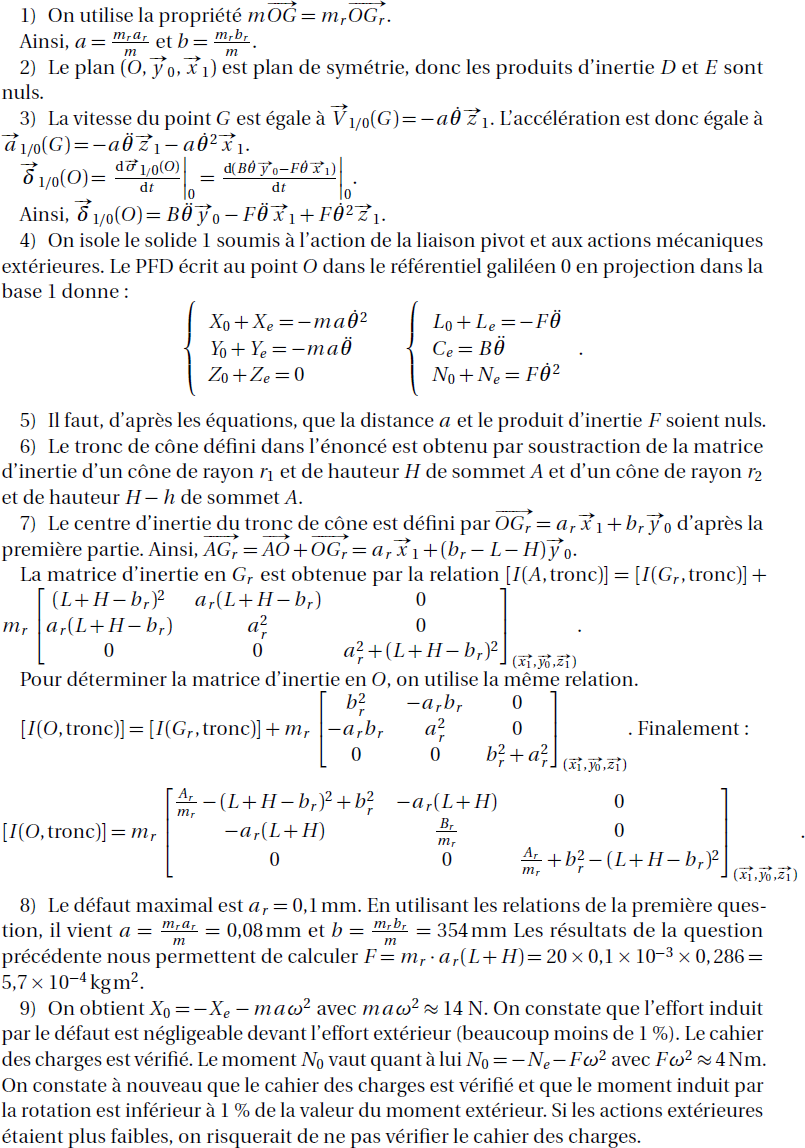
\includegraphics[width=.8\linewidth]{cor_01.png}
\end{center}
\begin{center}
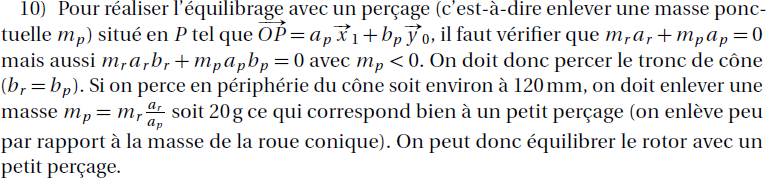
\includegraphics[width=.8\linewidth]{cor_02.png}
\end{center}

\else
\fi
